The \emph{Peer Manager (PM)} is a fundamental building block of the SmartSociety platform, providing a peer-centered data store that maintains and manages information about human- or machine-based peers within a privacy-preserving framework. 

\subsection{Mechanisms and algorithms}
%\todo{Peer Manager Theory - including flow diagram, pseudo-code if needed, whatever explain how it works}

The PM was designed as an extension of the notion of existing identity management systems\footnote{\url{https://en.wikipedia.org/wiki/Identity_management_system}}, with the objective of keeping the information owned by peers private.
In order to provide a flexible management of information, the PM builds upon the notion of an \emph{entity-centric semantic enhanced model} that defines an extensible set of entity schemas providing the templates for an attribute-based representation of peers' characteristics~\cite{Giunchiglia_fromknowledge}. Additionally, the PM defines a \emph{storage and privacy protection model} by adding privacy regulations and considerations~\cite{Hartswood:2015fe}. 
The design of this model pays special attention to different privacy issues discussed by the Council of Europe in its recommendation {\sc{cm}}/{\sc{rec}}(2010)13 on profiling \cite{CoE2010}, as well as 
basic legal privacy principles enacted by the {\sc{eu}} Data Protection Directive 95/46/{\sc{ec}} \cite{EUDir95} and that affects profiles when they involve the storage and processing of personal data.

An important feature of the SmartSociety PM model is that the concrete meaning of schemas is further specified by mapping single elements (i.e., types of entities, the names of attributes and their values) to concepts from an underlying ontology that is also part of the same model~\cite{Giunchiglia_fromknowledge}. This design provides additional flexibility in the operations supported, allowing reasoning over peer's properties as well as the implementation of semantic-enhanced services.
%
The basic set of schemas/templates can be easily extended to support new application-specific scenarios requiring, for instance, the creation of new types of peers. The adaptability is provided by enabling the search and information sharing services to work over the new types in a way that is transparent to the rest of the HDA-CAS platform.

%%% Privacy%%%
A key feature of the PM is that the privacy of peers is protected by allowing people (i.e. users) to define profiles that contain and reveal only partial or (semantically) obfuscated information that is used for replying to information requests from other modules/components and is thus enforcing data minimisation. 
This allows, for example, a human peer to reveal whether it is a smoker and its age range (as a way to obfuscate the age and date of birth) when participating in a ride-sharing collective, while the same information can be hidden (i.e., completely obfuscated) when participating in a question-answering collective.

%%% Architecture %%%
The details about the internal architecture of the PM was presented in~\cite{D4.2,Hartswood:2015fe}, however, we recall one of its main components (i.e., the Peer Base) in the conceptual view shown in Figure~\ref{fig:peerManagerPlatform}. The Peer Base is composed of the following sub-components: 
\begin{itemize}
\item A \emph{Platform-Wide Knowledge Base} (${KB}_{PW}$) that stores the core entity types and the underlying ontology, allowing interoperability among SmartSociety components. 
\item A \emph{Platform-Wide Entity Base} (${EB}_{PW}$) that stores entity instances of general interests as well as public profiles of peers (i.e., information that each peer decides to publish in the platform about themselves).
\item A \emph{Knowledge Base} (${KB}_i$) and an \emph{Entity Base} (${EB}_i$) for each peer, which store the peer’s information. The peer maintains control over its data space and defines the privacy policies that apply to the data stored in it. 
%The peer's $KB$ is bootstrapped with the content of the platform-wide's $KB$, which then can be extended/specialized by the peer. The peer's $EB$ stores entity instances that are relevant to the peer (i.e., peer’s personal information, its resources, locations, roles, tasks, etc.). 
\end{itemize}
This storage separation for each of the peers and the platform is one of the Privacy-by-Design decisions taken by WP4 in accordance to the PM  privacy protection model and to enforce privacy principles (such as data minimization, purpose specification and binding, consent). More information about the how structure and design decisions map to each of these principles may be found in D4.2.

\begin{figure}[t]
	\centering
	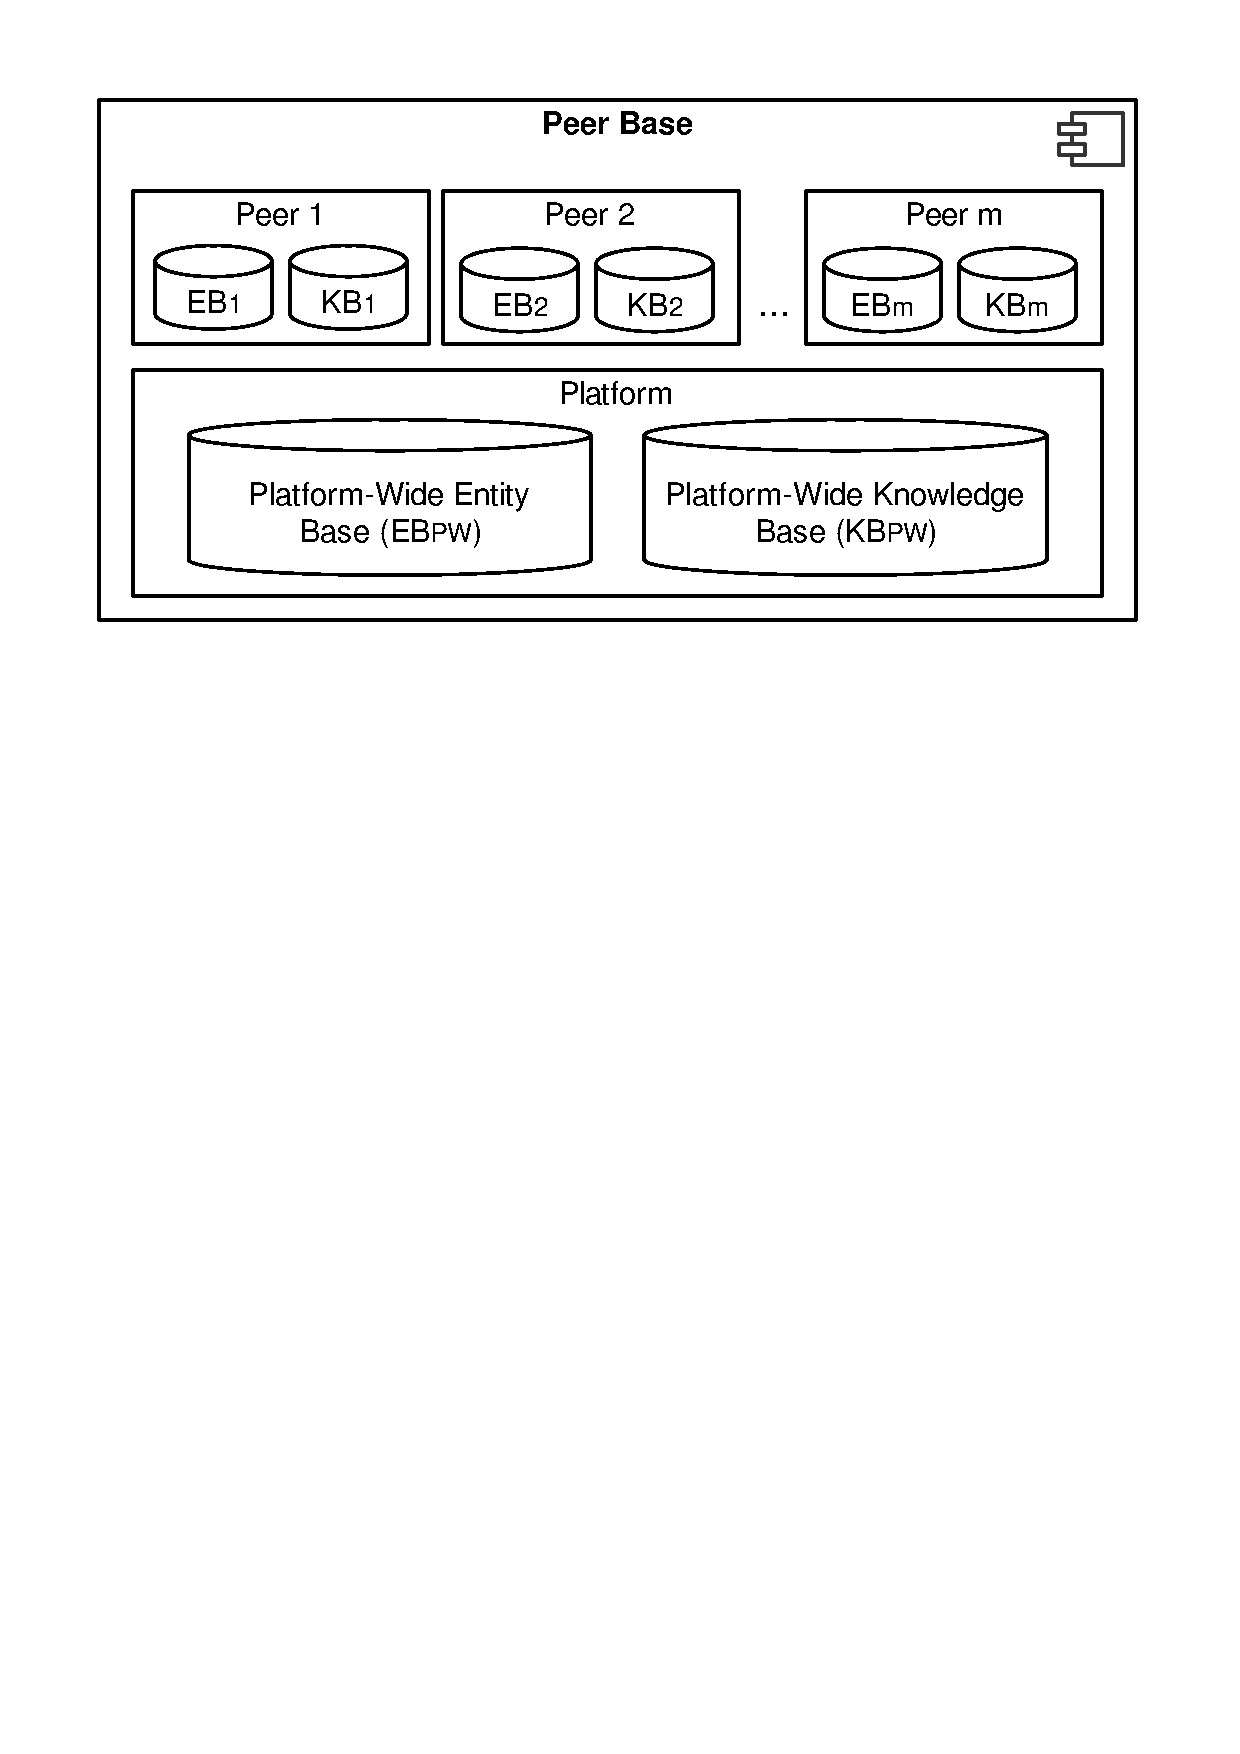
\includegraphics[width=0.65\linewidth]{figures/peerBase-diagram.pdf}
	\caption{Partial view of the Peer Manager internal architecture. Each subject its assigned its own peer storage, while the platform itself offers a shared Knowledge and Entity storages for different interactions.}
	\label{fig:peerManagerPlatform}
\end{figure}

\subsection{Implementation}
%{\it including how it has been implemented and specifications of APIs}

The Peer Manager component has been developed by following a three -layers approach, where each layer leverages the basic services offered by the level below and composes them for producing higher-level services. The resulting structure is shown in Figure~\ref{fig:pm-component-layers}; each layer will be further described in the remainder of this section. 

\begin{figure}[htbp]
\centering
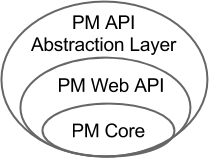
\includegraphics[width=0.3\textwidth]{figures/pm-component-layers.png}
\caption{Implementation layers of the Peer Manager}
\label{fig:pm-component-layers}
\end{figure}

\subsubsection{Peer Manager Core}
The Peer Manager Core provides a privacy-aware semantic storage for the SmartSociety Platform. This back end layer implements a semantic database and matching search facilities by using Java, the Hibernate and Spring Java frameworks, and the PostgreSQL database.

While these technologies represent previous work from the University of Trento, the SmartSociety (through the work documented in~\cite{D1.1,D4.1,D4.2}) has created the Knowledge Model used for representing peers, users, profiles (i.e. personal information) and more generally managing the information for running an HDA-CAS.

No major changes have been done to the models or structures of the Peer Manager during the first half of Y-3 (so the research reported in previous deliverables still holds) but efforts to update these models to its final version will start in the second part of the year (as T1.4 restarts) and will have its results reported in Deliverable D1.3. No major changes are foreseen, so the underlying code and the exposed interfaces will likely be subject to minor revision only. 

\subsubsection{Peer Manager Web API} \label{ssec:pm-web-api}
This layer takes the Java classes that implement the Peer Manager Core and wraps them in HTTP API calls that serve as a basic interface that clients or other back-ends may call to have access to the services the Peer Manager provides. Figure~\ref{fig:pm-interaction-arch.png} shows the Peer Manager Web API and the other components of the Peer Manager as part of the SmartSociety architecture. 

\begin{figure*}[htb!]
\centering
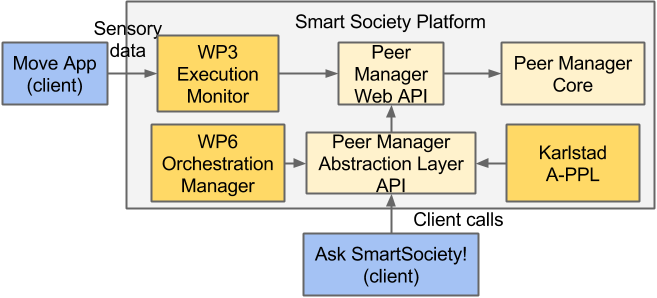
\includegraphics[width=1\linewidth]{figures/pm-interaction-arch.png}
\caption{Peer Manager Interaction Architecture. Arrow directions represent a component making a call or using a service from the other}
\label{fig:pm-interaction-arch.png}
\end{figure*}

In Figure~\ref{fig:pm-interaction-arch.png} the directed arrow from the Peer Manager Web API to the Peer Manager conveys that the Peer Manager Web API contacts exclusively the Peer Manager Core to answer to the requests it gets from the other components.

No major changes to the APIs described in~\cite{D4.2} were introduced in Y-3. API specifications for this layer may be found in the Appendix~\ref{sec:pm-web-api-detail}.

\subsubsection{Peer Manager abstraction layer API} \label{ssec:pm-abs-api}
The Peer Manager abstraction layer API is an additional level of abstraction that aggregates one or more of the calls from the previous layer into a single one to make the services offered by the Peer Manager easier to use directly from client applications and other SmartSociety platform components. The Peer Manager abstraction layer was developed for Node.js using languages like Coffeescript and Javascript. 

%Previous figure reference
Figure~\ref{fig:pm-interaction-arch.png} shows how a client application and some of the internal components on the SmartSociety Platform (Orchestration Manager and A-PPL) that are planned to interact with the Peer Manager, do so through the Peer Manager abstraction layer API. Furthermore, the directed arrow going out from the Peer Manager abstraction layer API shows that it uses exclusively the Peer Manager Web API to answer all requests.

%Comparison between calls from  the original API and this one
As an example of the type of abstraction done in this layer consider the abstraction layer API call used for creating a new peer within the Peer Manager (shown in Appendix~\ref{sec:pm-abs-api-detail}). This single call invokes the following calls in the Peer Manager Web API:
\begin{enumerate}
	\item Checks if the user name is taken
	\item Creates a new Peer structure and its main entity, which in this case is a Person entity (because this call is used to create new human peers)
	\item Creates a new User Entity that will represent that person in the system and connects it with the newly created Peer.
\end{enumerate}

Each of the steps in the previous procedure would take at from 1 to 3 calls if done directly from Peer Manager Web API, so this shows that Peer Manager abstraction layer API results in much more general and easy-to-use calls while still leveraging the full power of the Peer Manager.

Please note that this is a new component being developed specifically for the SmartSociety project and as such all code belonging to this layer will be open sourced. The under development API Specifications for this layer may be found in the Appendix~\ref{sec:pm-abs-api-detail}.

\subsubsection{Integration Approach with PPL policy language}

The Peer Manager theory presented in previous WP4 deliverables mentioned the need to include commonly agreed data handling policies between the source of the data (e.g. the person sharing the information) and the new data controller (e.g. the person that has received this information). Furthermore, one of the main novelties in the way that the Peer Manager handles access is that the system will be able to enforce directly the commonly agreed data handling policies (named "agreed requirements" inside the Peer Manager theory).

Previous iterations of the theory and architecture pointed that this would be done through integration of the Peer Manager and the Primelife Policy Language (PPL~\cite{PrimeLife534}) policy language but it is in this subsection where the first details and implementation details of such integration will be reported. 
In a close collaboration between WP4 and the University of Karlstad the following two approaches for integrating the PM (as defined in the D4.2 deliverable) and A-PPL engine (A-PPLE or A-PPL), which is Karlstad's current implementation of the PPL model, were defined:

\begin{enumerate}
	\item \emph{Basic integration approach}: the main idea of this approach is that both the PM and PPL run in parallel as different independent services and that they exchange information through their service APIs. In practice (and as shown in Fig.~\ref{fig:pm-ppl-lv1.png}) this will mean that the information in the Peer Manager profiles is not directly accessible (e.g. it is encrypted) and it is not readable without having access to the key being stored in a Pii (Personal Identifying Information) structure within the A-PPL system  (e.g. an encryption key). To authorize a request the A-PPL system will read the policy in the ``agreed requirements'' and evaluate the current request complies with them sending back only a ``allow'' or ``deny'' response to the PM. 
	\item \emph{Advanced integration approach}: in this approach both systems are still running independently in parallel  but the PM does understands how to read and enforce the agreed requirements encoded in PPL. The policies are still being created and stored in the A-PPL system and are dereferenced (as shown in Figure~\ref{fig:pm-ppl-lv2.png}) by the use of their identifiers.
\end{enumerate}

\begin{figure*}[htb!]
\centering
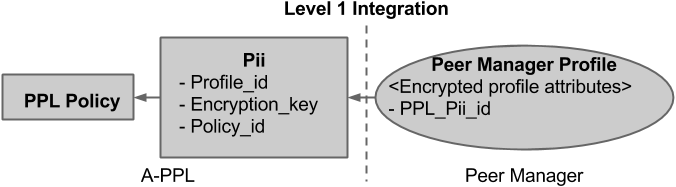
\includegraphics[width=0.8\linewidth]{figures/pm-ppl-lv1.png}
\caption{Basic Integration between the PM and PPL.}
\label{fig:pm-ppl-lv1.png}
\end{figure*}

Regarding the basic integration approach shown in Fig.~\ref{fig:pm-ppl-lv1.png}, it is important to note that the actual attribute information in the profile is not immediately accessible even to its owner (as explained in previous deliverables the PM model may choose to restrict the types of access that grants on profiles even to the owners of those profiles) and to read this information it needs the corresponding Pii entity stored in A-PPL (thus having to comply with the policy that protects the Pii). This is the simplest way to achieve integration while being absolutely sure that A-PPL authorizes the reading of the information in the Peer Manager Profile. Nevertheless, it is only suitable for test research purposes for the following reasons:
\begin{itemize}
	\item Time and space overhead of having the two systems running and parallel without acknowledging their close interaction. Even though both systems are made to run in the same server (to minimize possible overhead in their communication), for large volumes of data and users this overhead is bound to become significant
	\item Security issues, having only a single unchanging encryption\_key for each profile undermines purpose biding as you could ask access to the info for one purpose and then there is no system-level check preventing you from using the info for other purposes.
\end{itemize}

Even with the previous issue the basic integration approach has still value for Proof-of-Concept integration and for small testing exercises. 

\begin{figure*}[htb!]
\centering
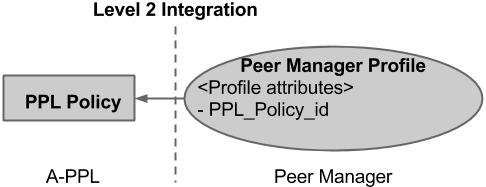
\includegraphics[width=0.6\linewidth]{figures/pm-ppl-lv2.png}
\caption{Advanced Integration between the PM and PPL.}
\label{fig:pm-ppl-lv2.png}
\end{figure*}

The mentioned problems are addressed within the advanced integration approach depicted in Fig.~\ref{fig:pm-ppl-lv2.png}. Here the A-PPL system is still used for the Policy storage and while the PM is supposed to have still no knowledge of how these policies are represented internally, the difference of this approach is that the PM does now understand how to enforce them. The Peer Manager will still ask the A-PPL system if a requested operation complies or not with a given policy, mainly because the PM does not share the same semantic ontology as A-PPL so it cannot know if a request complies with a Policy even if it has all information about both structures. This semantic heterogeneity is bridged through the mapping of the service APIs in both systems (the programmer doing the integration maps calls from one system to the other); and while this still requires the two systems still running independently in parallel, the space and time overheads are of less importance than those of the previous approach (as the Peer Manager already understand how PPL policies work but still needs to ask A-PPL to write and read these policies).

If needed, a third and final integration approach may be developed, involving the migration of the ontology that A-PPL uses for creating and interpreting the policies to the Peer Manager as a separate Knowledge Base (KB) belonging to a ``A-PPL peer''. Once this is done the Peer Manager will be able to support and enforce PPL without ever needing to call the A-PPL system, the A-PPL peer will then become a special privileged peer providing the service of writing and interpreting PPL policies within the SmartSociety platform. 

\subsubsection{Implementation of the Basic Integration Approach}
The current integration of the Peer Manager and PPL policies follows the `basic' integration approach described in the previous section. This means that both A-PPL and the PM services are running independently and interacting via HTTP calls. Furthermore, to minimize the communication overhead it was further decided that both services should run in the same server. 
%The implementation status of this integration is currently being tested and debugged to allow its use in future SmartSociety platform validation exercises.
 Specific details of the A-PPL calls being used by the PM for this integration can be found in the Appendix~\ref{sec:sec:a-ppl-api-detail} and below we present two examples of the flow between the two systems.
\begin{itemize}
	\item \emph{Creation of a Profile}: when the PM receives a request to create a new profile, it makes the following steps:
	\begin{enumerate}
		\item The Peer Manager creates the profile structure and uses the information passed along with the profile creation request for populating it.
		\item The Peer Manager encrypts all the content information within the profile. % (do note that currently a dummy encryption algorithm is being used but this can be replaced when using in testing systems).
		\item The Peer Manager sends a CreatePII call to A-PPL, containing the encryption key that can be used to unencrypt the profile, along with the policy requirements sent to the PM in the request for creating the profile. Upon receiving this information, the A-PPL will create a new Pii structure that will include the encryption key. Further, it will also create a new policy structure based on the policy requirements received from the PM that will restrict access to the previously created Pii.
		\item The Peer Manager receives back an identifier of the Pii created in A-PPL and stores it unencrypted in the source profile for future referencing.
	\end{enumerate}
	\item \emph{Reading of a Profile}: when a request for reading information of a profile is received by the Peer Manager, the following steps are undertaken:
	\begin{enumerate}
		\item The Peer Manager sends a getPII call to A-PPL, using the identifier of the Pii stored unencrypted in the profile (last step of the previous example) along with the details of the purpose of the read request.
		\item If A-PPL authorizes the previous request, it returns the encryption key to the PM and the profile information is unencrypted (otherwise a negative message is passed and the request fails).
		\item The Peer Manager answer the request with the least amount of information necessary to address it.
	\end{enumerate}
\end{itemize}